\documentclass[a4paper,oneside,article]{memoir}
\usepackage[T1]{fontenc}
\usepackage{textcomp}
\usepackage[utf8]{inputenc}
\usepackage[danish]{babel}
\usepackage[garamond]{mathdesign}
\usepackage{url}
\usepackage{graphicx}
\usepackage{pdflscape}
\usepackage{longtable}
\usepackage[draft]{fixme}
\usepackage{hyperref}
\usepackage{memhfixc}
\usepackage{listings}

\DeclareTextFontCommand{\textfleur}
{\fontencoding{T1}\fontfamily{FleurCornerCaps}\selectfont}


\renewcommand{\ttdefault}{pcr} % bedre typewriter font
\renewcommand{\rmdefault}{ugm} % garamond


\lstloadlanguages{HTML}
\lstset{language     = ML,
        extendedchars= false,
        breaklines   = false,
        tabsize      = 2,
        showstringspaces = false,
        basicstyle   = \small\ttfamily,
        commentstyle = \em
      }


\usepackage{lettrine}

%\overfullrule=5pt

%\setsecnumdepth{part}

\title{Hjemmesideanalyse  \\ \small{Førsteårsprojekt}}

\author
{
  Gruppe 1:\\
  Troels Henriksen (athas@sigkill.dk)\\
  Jesper Reenberg (reenberg@kampsax.dtu.dk)\\
  Martin Dybdal (dybber@dybber.dk)\\ \\
  Vejledere: Dina og Kasper
}


\setcounter{tocdepth}{2}
\setcounter{secnumdepth}{2}

\pagestyle{plain}

\date{\today}

\begin{document}
\maketitle
\newpage
\tableofcontents*
\newpage

\fixme{forskellig brug af fx os f.eks.}

\chapter{Indledning}
\label{indledning}
Mange hjemmesider forfattes i dag uden omtanke for om sidens målgruppe
er i stand til at læse sidens indhold --- det sproglige niveau er
ganske enkelt for højt. Ydermere forfattes indholdet af mange
hjemmesider med primitive værktøjer (f.eks. simple tekstfelter direkte
på siden, eller simple skriveprogrammer), der mangler de
hjælpefunktioner som findes i almindelige skriveprogrammer. Dette
resulterer i at hjemmesider ofte indeholder flere stavefejl end
gennemsnitlige tekster\fixme{hvilke tekster?}. Disse mangler kan gøre hjemmesider sværere at
bruge for den tilsigtede målgruppe, og derved reducere deres
effektivitet, ligegyldigt hvad målet med siden så end er.

Baseret på denne problemstilling har vi implementeret et program,
designet til at bistå hjemmesideforfattere med at forbedre den
sproglige kvalitet af deres sider, hvad enten dette er ved at reducere
antallet at stavefejl eller at omskrive unødigt kompliceret tekst.

Denne rapport beskriver design- og implementeringsprocessen bag vores
løsning af problemet, en arbejdsproces der blev udført i forbindelse
med Førsteårsprojektet på DIKU i blok 4, 2007.

Vores program endte med at opfylde alle de vigtigste krav nævnt i
vores kravspecifikation, og tests og eksperimenter viste at det er i
stand til at udføre de opgaver vi kom frem til i vores analyse (se
sektion \ref{analyse}). For nærmere detaljer omkring programmets
endelige tilstand, se konklusionen i sektion \ref{konklusion}.

Det forventes at læseren af denne rapport har en hvis grad af teknisk
kompetence, har erfaring med programmering og har en overordnet
forståelse for sproget HTML\footnote{Et sprog der bruges til at
  beskrive struktur og indhold af websites}.

\newpage
\chapter{Konklusion}
\label{konklusion}

\newpage
\chapter{Problemformulering}
\label{problemformulering}
Formålet med projektet er at skabe et program der kan bistå med at
forøge læsbarheden og den tekstmæssige kvalitet af hjemmesider. Af
simplicitetshensyn understøtter vi kun sider primært skrevet på dansk,
og vi behandler kun hjemmesidens indhold, og ikke dens typografi og
design.

Baseret på en analyse af hvilken målgruppe et sådan program er bedst
egnet til vil vi udvælge en mængde af features, som vi både mener er
realistiske at implementere på den afsatte tid, og som vil være
brugbare for projektets målgruppe.

\newpage
\chapter{Analyse}
\label{analyse}
I dette afsnit vil vi beskrive de tanker vi gjorde os omkring
problemet, og de forskellige løsningsmuligheder vi vurderede.

\section{Målgruppe}
\label{målgruppe}
Der er adskillige mulige målgrupper og en løsning på problemet kunne være
orienteret imod --- fra hjemmebrugere der skriver personlige sider,
over de individuelle skribenter på et større website til selve
webmasteren på en stor side. Ydermere kan et websites indhold
fortolkes på flere forskellige måder --- enten som almindelig tekst
omgivet af HTML-data uden betydning, eller med et forsøg på at benytte
den information som HTML-strukturen udtrykker. Sidstnævnte gør det
væsentligt lettere for et program at undersøge indholdet på et
website, idet mere information om sidernes indhold så er eksplicit
udtrykket i sidernes kode, i stedet for at programmet skal
``gætte''. Dette har også relevans i forhold til målgruppen, idet
HTML's avancerede features for at udtrykke semantisk information
omkring teksten (information om sprog, forkortelser, osv) primært
benyttes af tekniske brugere, og det virkede paradoksalt at lave en
løsning til ikke-tekniske brugere der virker bedst med data produceret
af tekniske brugere. Vi besluttede os for at det ville være et spild
at undlade at udnytte HTML's muligheder for at angive semantisk
information omkring teksten, men da en så lille del af verdens
websites benytter sig af HTML's muligheder indenfor dette område,
ville det heller ikke være hensigtsmæssigt at handikappe programmet
til kun at virke acceptabelt på denne form for HTML. Vores endelige
målgruppe endte med at blive todelt --- webmastere og
(semi-)professionelle skribenter. Dette valg baserer vi på at både
webmastere og skribenter har en stor interesse i at deres sider eller
tekst er let at læse, og har motivation til at sætte sig ind i
hvorledes man skriver god HTML, og derved gør det muligt for et
program at foretage en så god undersøgelse af websitet som
muligt.\footnote{Det kan nævnes at HTML-sider rig på semantisk
  information også gør det lettere for brugere af alternative
  weblæsere, som f.eks. blinde der benytter sig at netoplæsere, at
  benytte sig af siden} De, der ikke har interesse eller motivation
til at sætte sig ind i teknikken, har sandsynligvis også mindre
interesse i at deres websites er lette at læse --- ejerne af
professionelt orienterede websites har en væsentligt større interesse
i at deres sider er let læsbare end forfatterne af f.eks. en families
hjemmeside.

\section{Overvejelser omkring brugsscenarier}
\label{brugsovervejelser}
Vi blev hurtigt enige om at det er langt mere interessant at analysere
et website som helhed, end kun at analysere en specifik HTML-side, og
samtidigt at det er en nødvendighed at løsningen kan gennemgå
(``crawle''\footnote{\url{http://en.wikipedia.org/wiki/Web_crawler}}) et online website, og ikke være afhængig af at det i
forvejen er hentet og er beliggende som filer på brugerens
harddisk. Hvor det er relativt nemt at få et program, der kan
analysere et helt website, til kun at analysere en enkelt side, er det
omvendte langt sværere, idet man så skal implementere crawling seperat
fra programmet. Ydermere er især den ene del af vores målgruppe ---
webmastere --- sandsynligvis langt mere interesserede i at
analysere hele det website de er ansvarlige for, for at finde ud af
hvilke undersider der er uacceptabelt svære at læse, end at analysere
enkeltsider. Idet vi let kan forestille os at det kan tage lang
tid at analysere alle undersider på et stort website, forestiller vi
os også et brugsmønster hvori programmet automatisk bliver kørt med et
fast interval, og producerer et resultat som er tilgængeligt for alle
der arbejder på siden. Dette er langt mere effektivt end at alle
skribenter hver især skal køre tidskrævende analyser hver for sig. Dog
opfatter vi det også som sandsynligt at skribenter, der arbejder på at
forbedre læsbarheden af en specifik underside, vil have en mulighed
for hurtigt at analysere denne side for at se resultatet af deres
ændringer, i stedet for at de skal vente på at den automatiske analyse
bliver kørt (og bliver færdig igen).

\section{Brugergrænseflade og resultatpræsentation}
\label{brugergraenseflade}
En løsning på opgavens overordnede problem kan formuleres som at
analysere et website og producere en eller anden form for resultat,
der indeholder information om dets læsbarhed. Der er flere forskellige
muligheder for hvorledes brugeren skal kunne sætte en analyse i gang,
og hvorledes brugeren skal præsenteres for resultatet, og det rette
valg afhænger primært af den valgte målgruppe. Valget af
resultatpræsentation har stor betydning for løsningen, idet både valg
af teknologi, udformning af design og strategien for den endelige
implementation bliver påvirket hvorledes brugeren skal præsenteres for
resultatet. Der er også forskel på hvor godt forskellige
brugergrænseflader gør det muligt at analysere hele websites,
automatisere kørsel af programmet eller dele resultatet med andre
brugere (så hver bruger ikke skal køre en ny analyse fra start
af). Forskellige muligheder blev overvejet:

\begin{description}
\item[Integreret med webbrowser:]
  Programmet kan være en del af brugerens webbrowser --- når
  programmet er aktivt vil det, når brugeren besøger en side, indikere
  læsbarheden af siden. Dette kan ske på forskellige måder --- når
  brugeren holder musen over en sætning eller et afsnit kan f.eks. et
  LIX-tal (eller lignende) vises, et panel kan komme til syne i siden
  af browseren der indeholder information om sidens læsbarhed, eller
  teksten på siden kan farves efter hvor svær den er at læse. Fordelen
  ved denne løsning er at den er en udvidelse af brugerens normale
  brug af Internettet, og at information om læsbarheden af en given
  side præsenteres sammen med selve siden, og derved gør det let at
  forbinde læsbarhedsresultatet med sidens indhold. Det føles
  naturligt og intuitivt at bevæge sig ned af en side og lede efter
  indikerede problemer. 

  Ulempen ved denne præsentationsform er at det ikke umiddelbart lader
  sig gøre at analysere et helt website og kun søge detaljeret
  information om de mindst læsbare sider. En anden ulempe er at
  integrationen med browseren kan gøre det svært at automatisere
  kørslen af programmet, og at en præsentation der foregår i
  forbindelse med browserens egen visning af siden kan gøre det svært,
  for ikke at sige umuligt, at gøre resultatet tilgængeligt for andre
  brugere.

\item[Webapplikation:]
  Programmets brugerinterface kan være udformet som et website (en
  webapplikation), hvor brugeren kan angive adressen på et andet
  website, som så bliver analyseret. Præsentationen af resultatet
  kunne være en dynamisk genereret kopi af websitet, som brugeren kan
  navigere igennem online som hvis det var det oprindelige website,
  men hvor der på hver side er indsat information om tekstens
  læsbarhed. 

  Problemet med denne mulighed er at en komplet analyse af et
  middelstort website sandsynligvis tager længere tid end de fleste
  brugere er villige til at vente på, at en hjemmeside generer. Og der er ikke
  en umiddelbar måde at dele resultatet med andre brugere på.

\item[Grafisk standalone-applikation:] 
  Præsentationen kan udføres omtrent som nævnt i første mulighed, men
  i stedet for at køre som en del af webbrowseren, er det et vindue
  for sig selv, og det er selv ansvarligt for at vise indholdet af en
  analyseret side og sætte det i forbindelse med
  analyseresultatet. Hvis brugeren ønsker at analysere et helt website
  kan dette også gøres ved at programmet systematisk følger links på
  websitet og analyserer hver side det finder. Der kan så produceres
  en liste over de analyserede sider, hvorfra brugeren kan vælge at få
  mere detaljeret information (f.eks. den førnævnte visning af siden
  med uacceptabelt svært læsbar tekst markeret). Denne liste kan
  eventuelt sorteres efter sidernes læsbarhed eller lignende.

  Denne løsnings primære problem er at det er relativt svært at
  automatisere grafiske programmer, og at det stadigvæk ikke
  umiddelbart er muligt at dele et analyseresultat med flere
  brugere. En løsning på dette problem kunne være at opdele programmet
  i to dele --- en del der udfører den konkrete analyse og laver
  resultatet som en fil eller lignende, og en del der visuelt kan vise
  resultatet ud fra denne fil. En variant over dette er hvad næste
  mulighed går ud på.

\item[Output i form af HTML:]
  Programmet kan som foreslået ovenfor være konceptuelt opdelt i
  to --- en del der ``crawler'' et website og producerer et
  analyseresultat, og en del der giver en visuel præsentation af
  resultatet for brugeren. Dog er finessen at den første del
  præsenterer et sæt af HTML-filer, som kan læses af enhver
  webbrowser, hvilket betyder at vi ikke har behov for at implementere
  præsentationsdelen af løsningen. Programmet skal blot producere
  HTML-filer indeholdende websitets oprindelige tekst i forbindelse
  med analyseresultatet, og gøre det muligt at se alle undersider på
  websitet (f.eks. ved at producere en HTML-fil der indeholder en
  liste over alle de sider programmet besøgte under kørslen). Idet
  programmet ikke har behov for selv at præsentere resultatet visuelt
  (det håndteres af brugerens webbrowser) kan det implementeres som et
  kommandolinjeprogram, hvilket gør det nemt at automatisere, og da
  programmets output er almindelige HTML-filer kan disse nemt gøres
  tilgængelige for andre brugere.
\end{description}

Vi valgte sidstnævnte mulighed, og valgte også at implementere
løsningen som et kommandolinjeprogram. Dette sikrer et af vores
brugsscenarier, hvori programmet køres med et regulært interval og
producerer resultater der er tilgængelige for alle der arbejder på
websitet, og samtidigt er vi overbeviste om at det er muligt at lave
et så simpelt kommandolinjeinterface at skribenter hurtigt også kan
lære at bruge det. At output er i form af HTML-filer gør det også
muligt at lave nogle senere udvidelser eller alternative
brugergrænseflader --- en interessant idé kunne være en webapplikation
hvori brugere kan ``bestille'' analyser, og få en email med et link
til den producerede analyse (programmets output i form af HTML) når
den er færdig.

\section{Konkrete features}

Idet vores primære brugsscenarie omhandler analyse af alle sider på et
helt website tilgængeligt online (se sektion \ref{brugsovervejelser}),
er vores program nødt til at kunne lave en
forbindelse til en webserver, hente en HTML-fil, forstå indholdet af
HTML-filen, udføre en analyse af teksten i filen og følge hyperlinks
angivet i HTML-filen til andre sider på websitet. At følge hyperlinks
fra side til side er vores eneste mulighed for at besøge alle sider på
websitet, hvilket giver mulighed for at der findes isolerede sider som
vi ikke er i stand til at besøge, men da menneskelige besøgende på
siden også er nødt til at følge hyperlinks for at komme omkring, og
det derfor er yderst sjældent at der findes sådanne isolerede sider på et
website, mener vi ikke at dette er et problem.

\subsection{Indgrænsning af analysen}
\label{begraensning}
Der er mange faktorer der har indflydelse på læsbarheden af en
hjemmeside - fra tekstens indhold over de typografien og det visuelle
design, og selv valget af teknologi kan have indflydelse på
læsbarheden for visse brugere --- en side skrevet i Flash eller Java
kan f.eks. ikke benyttes af blinde der bruger netoplæsere. Indenfor
tidsrammen fandt vi det urealistisk at forsøge at vurdere siders
læsbarhed baseret på andre kriterier end selve teksten, så dette er
det eneste programmet inddrager i vurderingen af en sides læsbarhed
(dette afspejler sig også i problemformuleringen, se sektion
\ref{problemformulering}).

Udover at angive indhold og grafik kan HTML-sider også indeholde
\textit{scripts} --- \textit{ECMAScript} (også kendt som
\textit{JavaScript}) er det mest udbredte --- og disse scripts kan
under visningen af siden indsætte yderligere indhold på siden, ofte
som respons på brugerinput. For tiden er det faktisk moderne at
opbygge et helt website som en enkelt side, der baseret på input fra
brugeren dynamisk ændrer indhold uden at genindlæse hele siden fra
webserveren. Igen vurderede vi at vores program ikke ville være i
stand til at understøtte denne form for sider, idet den eneste
korrekte implementation ville være en komplet
\textit{JavaScript}-fortolker, kombineret med simuleret brugerinput,
en opgave som vi anslog til alene at ville tage \textit{væsentligt}
mere tid end de afsatte 7 uger.

Vi vælger altså derfor at begrænse os til kun at håndtere tekst der
findes direkte i HTML-siderne, men dog at understøtte alle nuværende
eksisterende versioner af HTML og XHTML (HTML skrevet i XML), dog ikke
alle features i XML, idet disse sjældent bruges i XHTML-sider (se
sektion \ref{htmlparserimpl}). Vores understøttelse af XML er
begrænset til den del der ligner SGML, og vi håndterer derfor ikke
namespaces\footnote{\url{http://www.w3.org/TR/REC-xml-names/}},
DTD'er \footnote{\url{http://www.w3.org/TR/2000/REC-xml-20001006\#sec-prolog-dtd}}
eller andre avancerede features.

\subsection{Analysemetoder}
\label{analysemetoder}
For at analysere teksten på siderne valgte vi at benytte to
analysemetoder -
læsbarhedsindeks\footnote{\url{http://www.elkan.dk/lixtal.asp}} og
FKRT\footnote{\url{http://en.wikipedia.org/wiki/Flesch-Kincaid_Readability_Test}}.
Læsbarhedsindeks (herefter refereret til som LIX) er en klassisk
algoritme til at analysere læsbarheden af en tekst, den er velforstået
af mange og virker derfor som et godt valg til programmet. Ydermere
har vi også valgt at benytte os af FKRT, der primært bruges til
engelsk tekst, men som også producerer brugbare resultater for dansk
tekst. Desuden fandt vi det også relevant at foretage stavekontrol af
de analyserede sider, idet mange sider bliver skrevet med primitive
værktøjer der ikke indeholder automatisk stavekontrol (se sektion
\ref{indledning}). Vi har nævnt at det er oplagt at benytte os af den
information som en sides HTML fortæller om dens tekst (se sektion
\ref{målgruppe}), og det er i forbindelse med stavekontrollen især
nærliggende at inddrage HTML's \texttt{lang}-attribut, som angiver en
teksts sprog, således at vi altid bruger den rigtige ordbog til at
stavekontrollen. Det gør det muligt for vores program at fungere med
sider der indeholder tekst skrevet på flere sprog, uden at det
ukorrekt angiver forkert stavede ord. Slutteligt taler vores egen
erfaring for at en hændelig skrivefejl er fejlagtig gentagelse af ord,
så denne fejl valgte vi ligeledes gøre opmærksom på (skriveprogrammer
med grammatikkontrol fanger denne fejl, men det gør en selvstændig
stavekontrol, som den i vores program, ikke).

\subsection{Overvejelser omkring output}

Som nævnt i sektion \ref{brugergraenseflade} består programmets output
af HTML-filer --- disse filer skal kommunikere resultatet på en
forståelig måde, idet de skal kunne stå alene når de ses i en
browser. Vi fandt det mest intuitivt at programmet laver en fil med
analyseresultater for hver side det besøger, og slutteligt laver en
overordnet indeks-fil der indeholder en liste over alle de besøgte
sider samt links til de filer, der indeholder detaljerne omkring
analysen af siderne. Disse sider indeholder den relevante sides tekst,
samt talværdier der angiver sidens læsbarhed (LIX-tal, FRE-tal og
FKGL-tal). Teksten på siden er opdelt i afsnit\footnote{I vores
  program dækker begrebet ``afsnit'' både over HTML's koncept om
  afsnit, adskilt af \texttt{p}-tags, samt over anden selvstændig
  tekst, som er strukturelt separat i HTML-dokumentet}, og for hvert
afsnit optræder der igen information om afsnittets læsbarhed --- dette
er for at gøre det lettere at finde, og få rettet, de mindst læsbare
afsnit på en side. Hver enkelt sætning har også en værdi associeret
med sig, der angiver hvor læsbar sætningen er --- men eksperimenter
viste at det var uholdbart at præsentere sætninger med tre tilknyttede
talværdier, på samme måde som med afsnittene, idet det ødelagde flowet
i teksten, og gjorde det trægt og besværligt at læse analysesiderne
igennem. Derfor bliver læsbarheden af sætningerne i et afsnit i stedet
indikeret via deres baggrundsfarve, som går fra lysegrøn for meget
læsbare sætninger, til blodrød for ulæselige sætninger. Vores
oplevelse er at farverne hurtigt gør det muligt at skimme en
analyseside og identificere afsnit der ser ``meget røde'' ud, uden at
man har behov for at gennemgå alle afsnittenes analyseresultater for
at finde den med den dårligste værdi.

HTML-dokumenter kan indeholde ``skjult'' tekst (herefter refereret til
som \textit{beskrivelser}), som f.eks. beskrivelser af links og
billeder, som ikke passer direkte ind i sætningsstrukturen. Idet denne
tekst også er relevant at medtage i resultatet bliver der efter hvert
afsnit vist en liste med beskrivelser fra afsnittet. Da denne tekst
kan fremkomme midt inde i en sætning fandt vi det ikke passende blot
at indsætte teksten hvor den er skrevet i HTML-dokumentet, og den
anden mulighed, at simulere hvordan teksten fungerer i det oprindelige
dokument ved først at vise den når man holder musen over sætningen der
indeholder den, ville skjule disse sætninger og deres farve fra en
hurtig skimning af analysesiden. Ovenfor blev det beskrevet hvordan en
sådan farvefølsom skimning er en af de mest praktisk måder at gennemse
et analyseresultat på, så en sådan løsning fandt vi uacceptabel. At
præsentere beskrivelserne som en liste efter selve afsnittets tekst
betyder at det er sværere at kode den sammen med den egentlige tekst i
HTML-dokumentet, men idet beskrivelserne i listen har samme rækkefølge
som beskrivelserne på den oprindelige side, og fordi der ofte er
relativt få beskrivelser i et afsnit, mener vi ikke at dette er et
stort problem, og vi mener at denne løsning er at foretrække frem for
de alternativer vi overvejede.

Programmet understøtter flere features, især omkring
indstillingsparametre og håndtering af specifikke HTML-tags, men disse
er ikke analysemæssigt særligt interessante, og vi henviser derfor til
den vedlagte kravspecifikation for en mere detaljeret gennemgang.

\newpage
\chapter{Programdesign}

For at gøre implementationsfasen af projektet så nem og effektiv som
muligt har vi udformet et design der angiver programmets overordnede
struktur, dog uden at gå i for mange konkrete detaljer. Dette sikrer
at designet både fungerer som en vejledning under implementationen,
men ikke behøver revision hvis der under implementationen opstår
komplikationer som det oprindelige design ikke tog højde for. Derfor
vil vi beskrive centrale datastrukturer og algoritmer på et abstrakt
plan, men ikke angive f.eks. konkrete typer eller beskrive deres
konkrete implementation eller interface.\fixme{eventuel henvisning til hvor den konkrete implementetion bliver beskrevet ??}

Dette afsnit vil beskrive det overordnede design vi valgte at
implementere vores program omkring, samt begrundelser for hvorfor
dette design blev valgt.

\section{Overordnet designfilosofi}
Vi har valgt at basere vores programimplementation på et
\textit{dataflow}--design, hvori fokus er hvorledes data bliver ført
rundt i programmets moduler. Idet vores program ikke er interaktivt,
men derimod kører som et \textit{batch--job} med en fra starten af
veldefineret afslutning (når alle sider er blevet analyseret), i
modsætning til interaktive programmer, som kører indtil brugeren
vælger at afslutte dem, er et dataflow--design velegnet, da vi kan
være sikre på i hvilken rækkefølge indkommende data skal behandles. Da
programmet ydermere er baseret på at foretage gradvist mere
raffinerede bearbejdninger af det indkommende data er et
dataflow--diagram velegnet til at vise hvorledes den i starten ``rå''
og ustrukturerede data bliver destilleret ned til den endelige analyse
via gradvist mere finkornede processer. Programmeringssproget Standard
ML er velegnet til en sådan opgave --- manglen på objektorienterede
faciliteter vil ikke blive mærket idet problemet og designet ikke
passer umiddelbart ind i den objektorienterede filosofi, og
programmets relativt korte og simple kørselstid betyder at der ikke er
et så stort behov for mutérbar tilstande. 

På figur \ref{dataflowdia} kan vores Dataflow diagram ses. Det primære
dataflow er angivet med solide linjer. Indstillingerne går uden om det
primære dataflow og er angivet med stiplede linjer.
\begin{figure}
  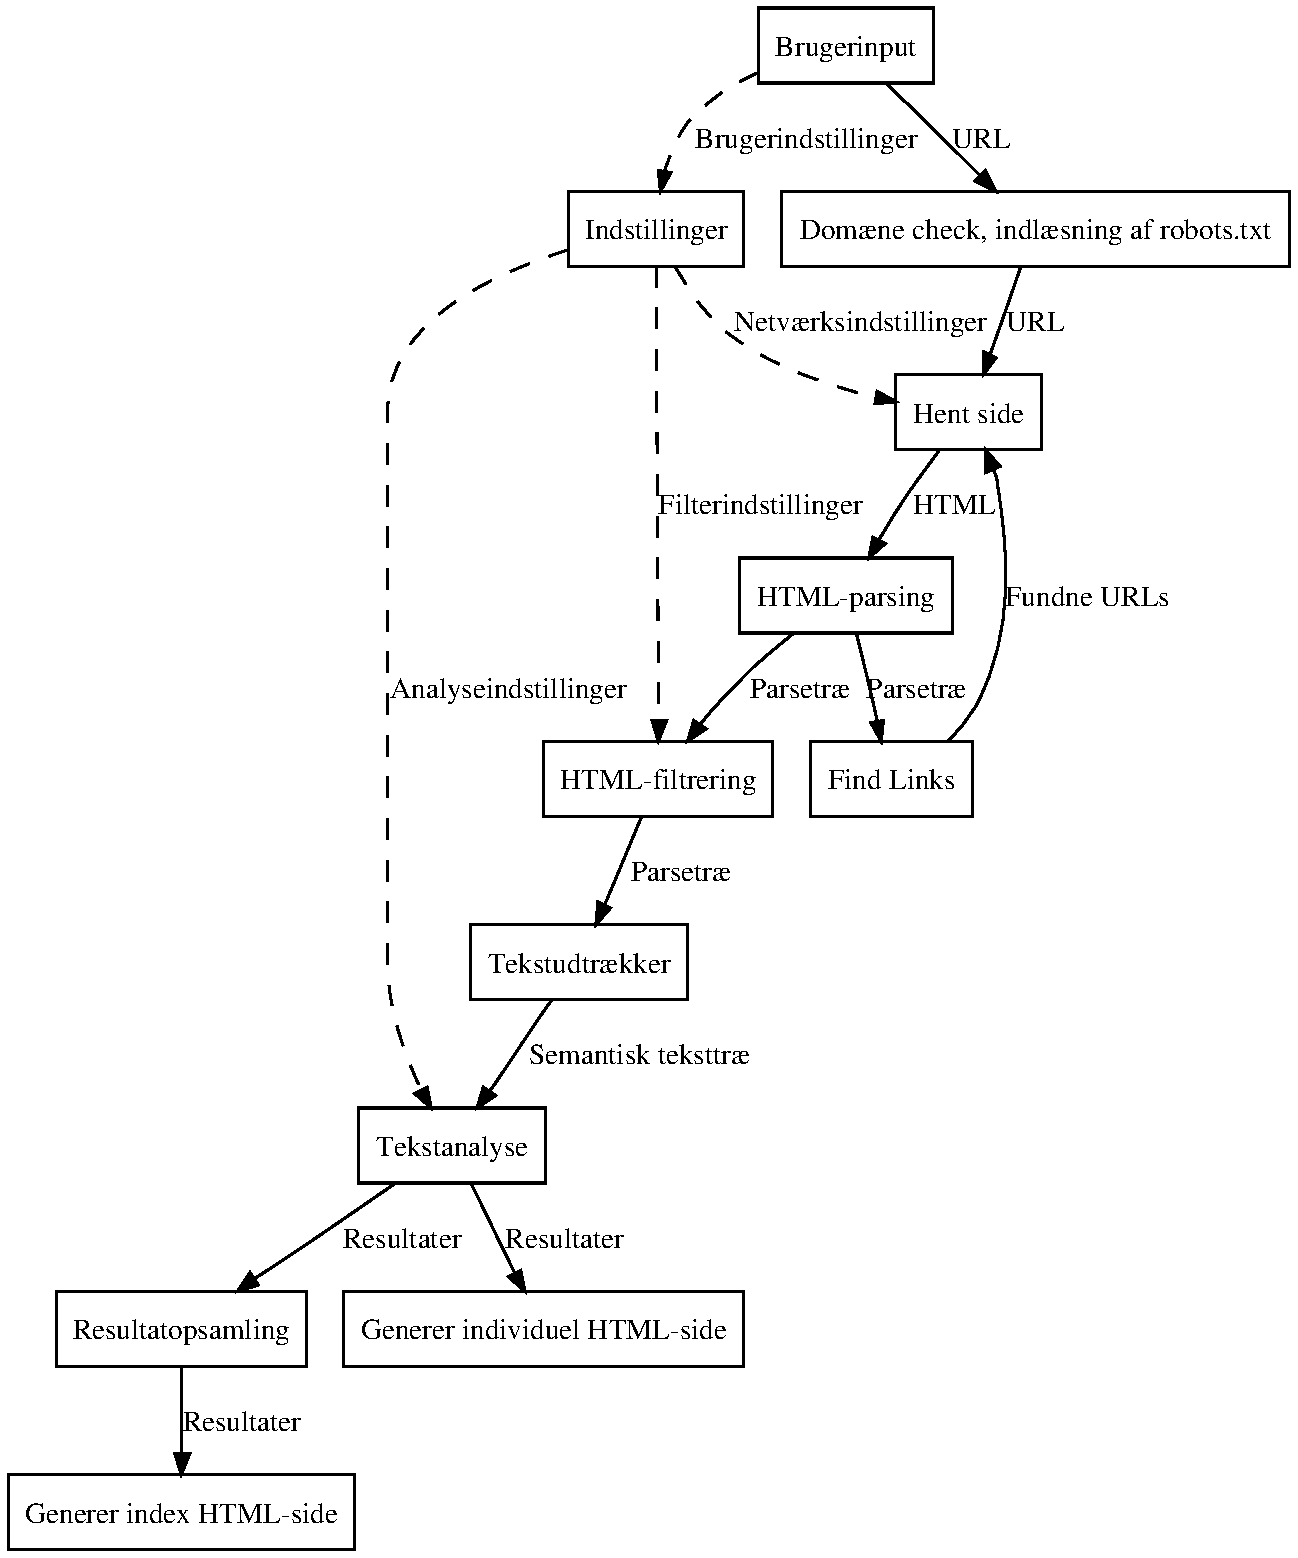
\includegraphics[width=\textwidth]{endeligtdesignill.pdf}
  \caption{Dataflow diagram}
  \label{dataflowdia}
\end{figure}

\newpage
\section{Moduler}
Vi vil nu beskrive de moduler vi har inddelt programmet i. I det
følgende henfører ``moduler'' ikke nødvendigvis til Standard ML's
modul--feature, selvom det ikke kan afvises at dette sprogkoncept vil
blive brugt til at implementere enkelte af dem.

\subsection{Brugerinput og brugervenlighed}
Dette modul skal sætte en analyse i gang ud fra de parametre brugeren
angiver. Det skal parse kommandolinjeparametrene og videregive
brugerindstillingerne til de andre moduler i programmet. Hvis
kommandolinjen er i et ugyldigt format, eller der er angivet ukendte
indstillinger, er det også dette moduls ansvar at informere brugeren
om fejlen og afslutte programmet.

\subsubsection{Brugervenlighed}
For at gøre programmet let at bruge, er det vigtigt at de
indstillinger man kan angive er lette at huske for brugeren. En bruger
vil hurtigt blive træt af at skulle slå op i manualen hver gang
programmet skal bruges. Når man starter programmet er der én
indstilling man \textit{altid} vil skulle angive --- startadressen for
analysen. Denne indstilling skal, som den eneste, ikke angives med et
specielt præfiks, netop fordi den er så vigtig. De andre indstillinger
angives med et præfiks f.eks. ``--l'' for angivelsen af sprog. Måden
disse indstillinger angives, er valgt ud fra at det skal være let at
sætte deres navn/præfiks i forbindelse med deres
betydning. Eksempelvis kan man angive hvor den maksimale dybde for
analysen med indstillingen ``--d'', hvor \textit{d}'et står for
\textit{depth}. Udover at det skal være let at huske sammenhængen mellem
betydning og navn, så skal tvetydigheder helst undgås. Tvetydigheder
kan gøre at brugeren husker forkert og føler det
nødvendigt at slå op i manualen. Når flere indstillinger kunne have
samme navn, har vi valgt at bruge et længere navn for at undgå
disse tvetydigheder. F.eks. er der to indstillinger der begge kan
angive at noget af dokumentet skal ignoreres i analysen, disse
indstillingers navne er ``--ignore--tag'' og ``--ignore--id''.

\subsection{Indstillinger}
Da de brugerleverede indstillinger skal kunne tilgås fra vidt spredte
dele af programmet har vi fundet det bedst at lagre disse på et
centralt, løst koblet sted, i modsætning til programmets egentligt
arbejds--data, der i højere grad fører data rundt gennem tæt koblede
moduler og typestærke interfaces. Dette sikrer også at det er
let at tilføje nye indstillingsmuligheder --- idet der kun skal ændres
i den kode der rent faktisk udnytter den nye indstillingsmulighed ---
hvor ændringer i det primære dataflow kan resultere i en kaskade af
ændringer over det meste af programmet. \fixme{Tekst der følger her giver ikke meget mening} Den uafhængige plads
indstillings---informationen har ville dog ikke være nær så passende
til den primære data, idet det ville gøre det sværere at kontrollere
hvor og hvornår den blev ændret, og ville svække muligheden for at
garantere den sekventielt løbende raffinering af arbejdsdata som
programmet er bygget op omkring.

\subsection{Domæne check, indlæsning af robots.txt}
Dette modul skal tjekke om det domæne brugeren har angivet kan tilgås
og give en fejlmeddelelse hvis det ikke er tilfældet. Hvis brugeren
har angivet det skal det undersøges om der er en
\textit{robots.txt}--fil (en standard, der gør det muligt for websteder
at bede søgemaskiner og andre robotter om at lade være med at besøge
dele af siden) \footnote{\url{http://www.robotstxt.org/}} på serveren
og hvis det er tilfældet så skal den parses. Informationerne i
\textit{robots.txt} skal gøres tilgængeligt for \textit{Hent
  side}--modulet, så det kan se hvilke dele af webstedet det må crawle.

\subsection{Hent Side}
Hent side modulet skal kunne hente en side fra en webserver via
HTTP--protokollen. Da vores behov er små og vi ikke har for meget tid
vil vi bruge et eksternt produceret
HTTP--modul\footnote{\url{http://www.diku.dk/undervisning/2000e/dat0/filer200001/K1/brevkasse.html}},
modificeret til vores behov. Det er også dette moduls job at tjekke om
den indlæste \textit{robots.txt} tillader at vi må crawle siden, da dette skal
tjekkes hver gang der skal hentes en side.

\subsection{HTML--Parsing}
\label{htmlparsing}
For at kunne udtrække tekst fra en HTML-side er det nødvendigt først
at parse den. Da vi ikke har været i stand til at finde en HTML--parser
skrevet i SML har vi valgt at implementere denne selv. Resultatet af
HTML--parsingen er et ordinært parsetræ som så i senere moduler bruges
til både at danne et mere højniveau--træ over teksten, og til at finde
links til andre sider som skal hentes.

Parseren er, for at lette implementationen, opdelt i to primære dele ---
en lexer, der opdeler den indkommende sekvens af tegn i en liste af
leksikalske enheder uden nærmere struktur, og en egentlig parser, som
omdanner listen af de leksikale enheder til et struktureret
parsetræ. Lexeren er specificeret med en SML--signatur, men det er ikke
hensigten at denne bruges af andet end parser--modulet, og resten af
programmet vil ikke være påvirket af parsertrinnets toparts--opdeling.

De leksikale enheder produceret af lexeren vil være af tre forskellige
typer --- begyndelsestags, afslutningstags og tekstelementer. De to
tag--typer vil indeholde information om navnet på det relevante tag,
samt en liste indeholdende attribut/værdi--tupler. Tekstelementer vil
indeholde information om den sekvens af tegn de repræsenterer.

Det af parseren producerede parsetræ består af knuder, repræsenterende
tags, og blade, repræsenterende tekst. En knude kan have nul eller
flere undergrene der angiver de HTML--elementer der findes mellem
start-- og slut--tagget (nul undergrene kunne f.eks. være et
``\texttt{<br />}''--element), hvor hver undergren igen kan være enten
en knude eller et blad. Undergrenene skal være ordnede i samme
rækkefølge som deres optræden i det oprindelige HTML--dokument. En
knude indeholder information om hvilket tag den repræsenterer, samt
eventuelle HTML--attributter tagget har.

For eksempel vil HTML--dokumentet på figur \ref{htmldoc1} give et
parsetræ, som det illustreret på figur \ref{parsetree}. På figuren er
børnene arrangeret så det første barn står længst til venstre og det
sidste længst til højre. Hvert tag har et sæt attributter, på figuren
er indholdet af disse dog udeladt. De fleste af attributsættene er
tomme, men som det kan ses i HTML--dokumentet så har
\texttt{BLOCKQUOTE}-- og \texttt{A}--tagsne en attribut hver.
I parsetræet er der også en del mellemrums--tegn der er ikke er
medtaget for at simplificere figuren.

\begin{figure}
\begin{lstlisting}[language=HTML]
<HTML>
<HEAD><TITLE>Sidetitel</TITLE></HEAD>
<BODY> <!-- En kommentar -->
  <P>Et afsnit med adskillige sætninger.
  Dette er 'den anden sætning'.</P>
  <BLOCKQUOTE lang="en">
    <A href="http://en.wikipedia.org/wiki/Hovercraft">My hovercraft</A>
    is full of eels!</BLOCKQUOTE>
  </BODY>
</HTML>
\end{lstlisting}

  \caption{Eksempel HTML--dokument.}
  \label{htmldoc1}
\end{figure}

\begin{figure}
  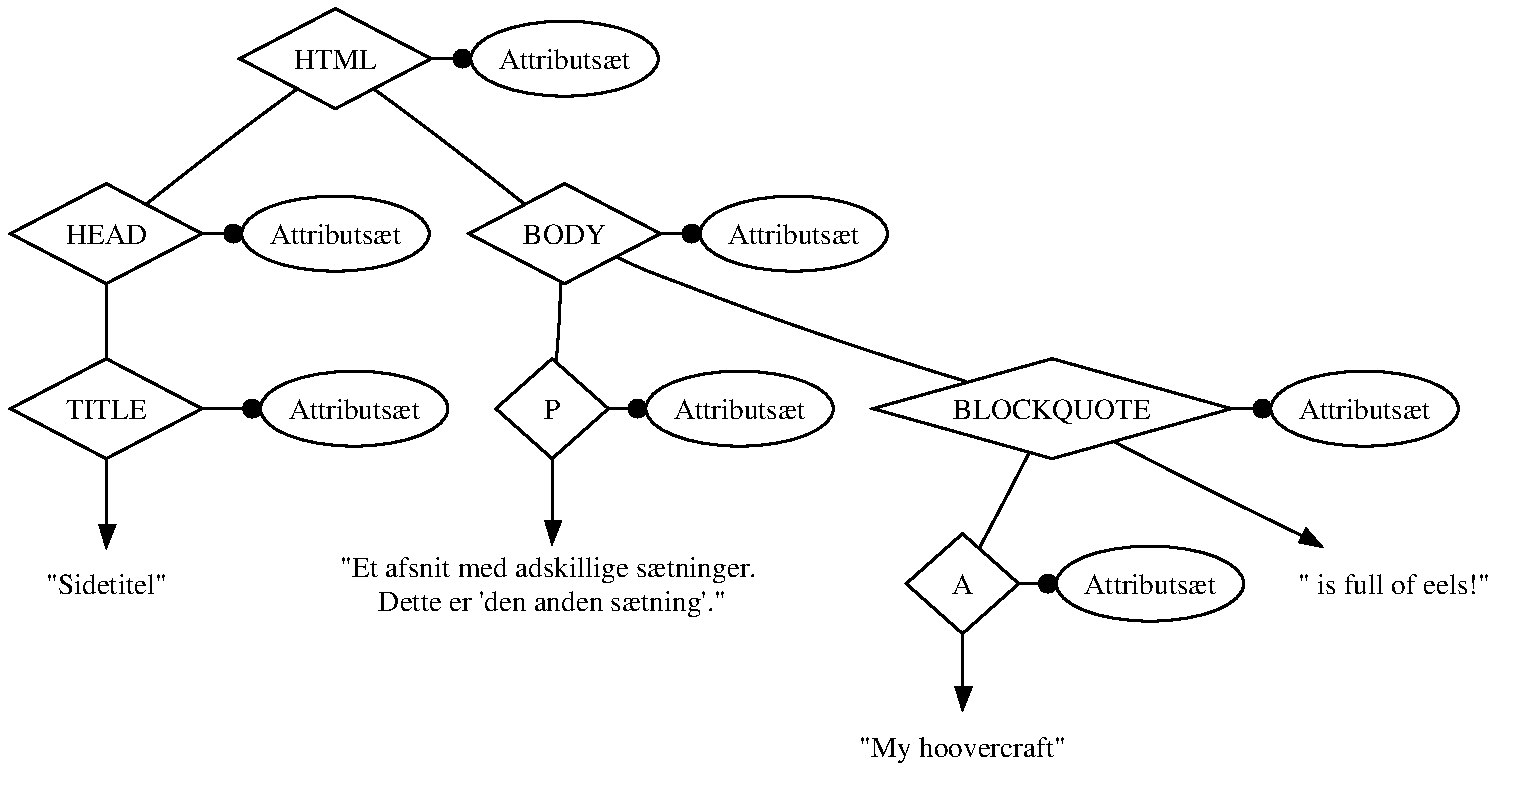
\includegraphics[width=\textwidth]{parsetree.pdf}
  \caption{Parsetræ for HTML--dokumentet på figur \ref{htmldoc1}.}
  \label{parsetree}
\end{figure}

\subsection{Find links}
Dette modul skal ud fra HTML--parsetræet genereret af HTML--parseren,
lave en liste af de links som linker til andre sider på samme domæne.
Det skal derefter bede om at disse sider bliver hentet, parset og
analyseret, og undersøge links på de nyhentede sider --- en rekursiv
proces der løber indtil alle tilgængelige sider er blevet analyseret.

For at finde linksene skal alle \texttt{a}--tags findes --- deres
\texttt{href} attribut angiver så det link der peges på. De adresser
man finder kan være relative til den nuværende side. Den absolutte
adresse til den nuværende side skal derfor kombineres med den relative
sti fra linket for at forme linkets absolutte sti. Det er dog ikke
altid den nuværende sides absolutte sti som adresser skal være
relative til, man kan angive en anden sti som de skal være relative
til med \texttt{base}--tagget. Da \texttt{a}--tags også bruges til andet 
end links til almindelige htmlsider, sørger vi for at filtrere dette fra. 
Dette kunne fx være links til mails \texttt{mailto:} eller javascript
funktioner \texttt{javascript:}

Det er ikke kun \texttt{a} der skal undersøges, hvis et HTML--dokument
benytter sig af rammer (frames), så skal deres start--adresser også
findes. Der er også andre tags der tillader at man specificerer
adresser til forklaringer ol, disse skal der også tages hån om.

På diagrammet går kun en enkelt pil fra ``Find links''--modulet til
``Hent side''--modulet. Reelt bliver denne pil fulgt for hvert eneste
fundet link som ikke allerede er blevet besøgt --- resultatet bliver at
cyklussen i diagrammet fungerer som programmets primære loop der
henter og analyserer links, indtil der ikke kan findes flere indenfor
den angivne maksimaldybde.

\subsection{HTML--filtrering}
For at gøre det muligt at angive at nogle dele af en hjemmeside ikke
skal analyseres er det nødvendigt med et modul der kan frasortere de
ønskede elementer fra siden. Ud fra brugerens indstillinger skal dette
modul kunne frasortere dele af en HTML--side. Dette kan fx bruges
til at frasortere menuer, brugerkommentarer og andet tekst som vil
kunne påvirke analysen, på en måde så resultatet bliver
misvisende. Beregningen af læsbarhedsindekset kan eksempelvis blive
påvirket af at der i menuer ofte er en stor andel lange ord.

\subsection{Tekstudtrækker}
Når et HTML--dokument er parset kan vi udtage teksten, det er dette
moduls job at læse parsetræet for et HTML--dokument og omdanne det til
afsnit, sætninger, overskrifter osv, som \textit{Tekstanalyse}--modulet
kan analysere. Udover at opdele teksten skal de enkelte tekstpassagers
semantiske betydning bibeholdes.

\begin{figure}
  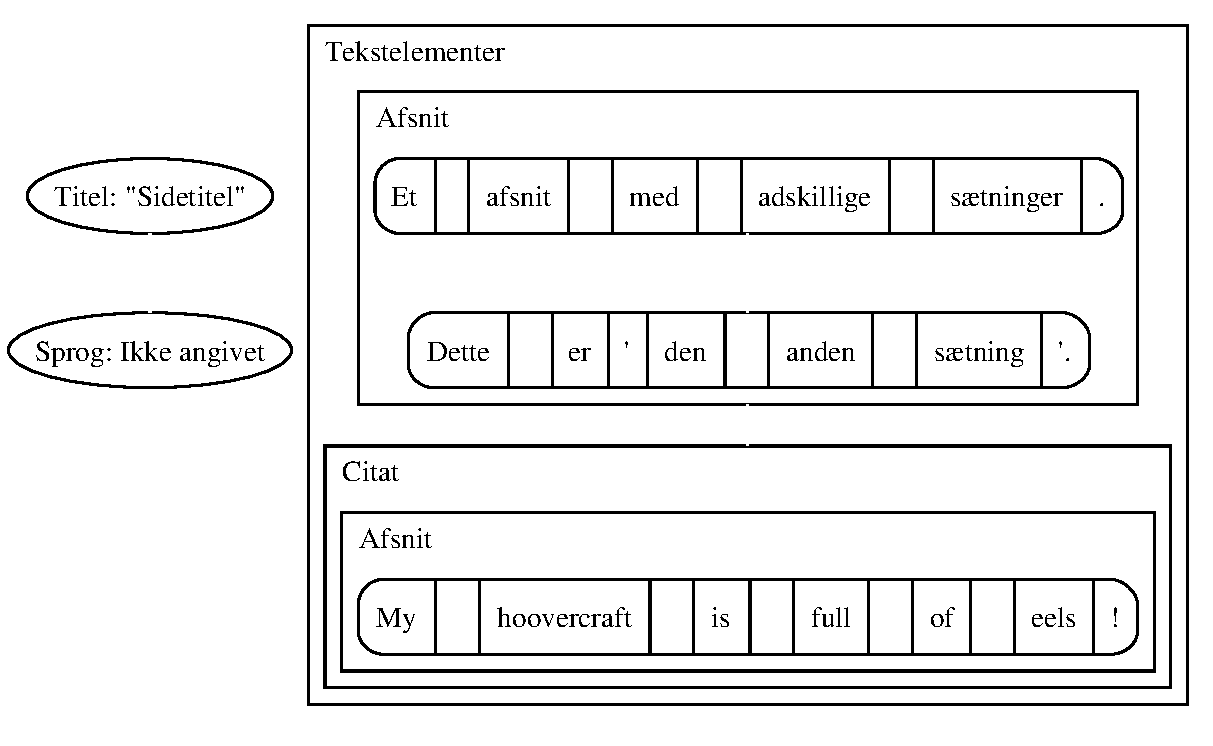
\includegraphics[width=\textwidth]{documentill.pdf}
  \caption{Resulterende dokument--struktur for parsetræet på figur
    \ref{parsetree}}
  \label{dokument}
\end{figure}

På figur \ref{dokument} er vist et eksempel på den resulterende
datastruktur. Dokumentet består af en titel, et sprog og en liste af
tekstelementer. Et tekstelement er enten en overskrift, et citat eller
et afsnit. Afsnittene er de mest interessante, da overskrifter og
citater i sig selv blot består af en liste afsnit. I HTML angives
afsnit med \texttt{P}--tagget, men der er også en række andre tags der
adskiller teksten i afsnit, f.eks. startes der et nyt afsnit efter et
billede, en tabel, faktisk sker det ved alle tags der er
``block--elementer''. Et afsnit består af en række sætninger og en
række ``ekstra'' sætninger som er den tekst der ikke umiddelbart
optræder på HTML--siden, men som alligevel er interessant --- såsom
\texttt{title} og \texttt{alt}--tekst for links og
billeder. Sætningerne er opdelt i ord og punktuering (tegnsætning,
mellemrum mv.) og hver sætning slutter ved et eller flere punktummer,
spørgsmålstegn eller udråbstegn. Hvert ord har semantisk
information fra HTML'en tilknyttet, som f.eks. information om hvorvidt
ordet er en forkortelse, eller oprindeligt har været inde i et
\texttt{em}--tag.

For ikke at låse programmet fuldstændig fast til HTML er dette modul
delt i to delmoduler. Det ene modul (den egentlige tekstudtrækker)
kender til selve HTML--formatet og omdanner det til en mere generisk
datastruktur der symboliserer et dokument. Denne datastruktur
indeholder information om tekstens inddeling i afsnit, overskrifter,
citater mm. Datastrukturen viderebehandles af det andet delmodul
(``sætningsifikatoren'')\fixme{sætningsifi hvad for noget ?}, som udfører de
beregninger der er ens for
alle dokumenter. Dette inkluderer adskillelse af ord og punktuering
(mellemrum, tegnsætning mv.) og opdeling i sætninger.  Det første
delmodul kan på denne måde let udvides så det også kan håndtere andre
dokumentformater.

\subsection{Tekstanalyse}
Her skal de egentlige analyser foretages, modulet får teksten fra
\textit{Tekstudtrækkeren} og udfører de af brugeren valgte
tekstanalyser.

Til beregning af både lixtal og Flesh Reading Ease skal bruges
informationer om bl.a. antal ord og antal sætninger. Det vil resultere
i dobbeltarbejde hvis flere analyser beregner disse tal, for at
afhjælpe dette vil vi lave en forudgående indsamling af informationer
om teksten, der kan være relevante for flere af analyserne. Dette vil
også lette arbejdet med evt. implementation af yderligere
tekstanalyser, da det i princippet kun er den matematiske formel der
skal indtastes, medmindre meget specifikke informationer ønskes
(Fx ``Hvor mange ord er der med 3 stavelser eller færre?'').

Uddata fra tekstanalysemodulet er en datastruktur der meget ligner
input, men som i stedet for semantisk information har fået tilknyttet
læsesværhedsgrad--data til de leksikale enheder (afsnit, sætninger og
ord).

Det er også i analysemodulet at ord stavekontrolleres baseret på deres
angivne sprog, og får tilknyttet en værdi der angiver om de er korrekt
stavet eller ej. Til at foretage selve stavekontrollen vil vi bruge
GNU Aspell\footnote{\url{http://aspell.net/}}. Vi mener ikke det er et
urimeligt krav til brugerens system at GNU Aspell skal være
installeret, da det er et relativt almindeligt program på
GNU/Linux-systemer (vor målplatform). For at gøre det muligt senere at
skifte til en anden type stavekontrol, er det bedst at denne
funktionalitet er adskilt så meget fra resten af programmet som
muligt. Vi vil derfor indkapsle stavekontrollen i sit eget delmodul,
som det egentlige tekstanalyse--modul kan forespørge.

\subsection{Generer individuelle HTML--sider}
Dette modul skal lave de HTML--filer der skal præsentere
analyseresultaterne for brugeren. Givet analyse resultaterne for en
enkelt side skal det generere en HTML side. HTML--siden vil få et
deterministisk navn baseret på HTML--filens navn og placering på
websitet, således at der kan skabes links til den genererede HTML--fil
fra analyseindekset. Til at generere HTML'en bruger vi et modul
baseret på Msp (ML Serverpages), dette er en del af Moscow ML's
standardbibliotek\footnote{\url{http://www.dina.kvl.dk/~sestoft/mosmllib/Msp.html}}.

\subsection{Resultatopsamling}
For hver side udregnes en sidesværhedsgrad som skal vises på
oversigtssiden for analyseresultatet. Dette modul skal gemme
sidesværhedsgrad for hver side, så der kan genereres en index fil når
analysen af alle undersiderne er afsluttet.

\subsection{Generer index HTML--side}
For at brugeren nemt kan få adgang til analyseresultaterne vil vi også
generere en index fil. Dette skridt er det absolut sidste der tages i
programmet, og først når alle websitets undersider er blevet
analyseret.

\section{Redegørelse for designets kvaliteter}
Ved at bruge dette design vil vi kunne indfri alle de krav der er
stillet i kravspecifikationen. Derudover vil designet gøre det nemt at
udvide programmet til at understøtte flere tekstformater og flere
analysemetoder.

Alle modulerne kan testes systematisk \fixme{Unit testing?}, måske med
undtagelse af
\textit{Hent side} modulet, da testen af dette modul kræver en
forbindelse til en webserver, som vi kan være sikker på ikke ændrer
indhold. Men fordi det at hente en side er meget veldefineret vil det
sandsynligvis ikke være et problem.

Den klare opdeling i moduler som udveksler data gør det muligt at
parallelisere udviklingen, således at de enkelte moduler kan
implementeres og testes for sig selv, uden at afhænge af en færdig
implementation af de andre moduler. Hvert konceptuelt modul kan, om
ikke fuldstændigt, så til en vis grad, implementeres som en SML
modulsignatur og struktur.

\newpage
\chapter{Implementation}

\section{Parsing af HTML}
\label{htmlparserimpl}
For korrekt at udtrække tekst, og information om teksten, fra et
website, er det nødvendigt at kunne parse HTML, eller have en anden
måde at adskille tekst fra tags og forbinde informationen i tags til
den tekst der står under dem. I vores program valgte vi at
implementere en nogenlunde fuldgyldig HTML parser (se nedenfor for
dens begrænsninger), da vi mente at det ville være lettere at udtrække
information fra et parse--træ, end hvad søgning med f.eks. regulære
udtryk ville resultere i. Blandt andet på grund af vores begrænsede
tidsresurser var der en række krav til parseren og dens
implementation:

\begin{itemize}
\item Den skal kunne håndtere både HTML og XHTML (se sektion
  \ref{begraensning}), idet vi ikke har tid til at implementere to
  forskellige parsere. Heldigvis minder HTML og XHTML meget om
  hinanden, og XHTML-sider udnytter sjældent XML's mere avancerede
  features, så vi valgte ikke at understøtte disse.
\item Vi valgte at undlade at forsøge at håndtere indholdet af
  \texttt{script} og \texttt{style}-tags korrekt, til trods for at
  indholdet af disse kan indeholde tekst der kan forvirre
  parseren. Grundet tidsnød valgte vi at undlade at implementere denne
  håndtering, et problem der er begrænset i omfang, idet størsteparten
  af moderne sider specificerer eksterne scripts og
  \textit{CSS--stylesheets}, hvis indhold altså ikke ligger direkte i
  HTML-dokumentet, og som derfor ikke kan forvirre
  parseren. \textbf{Dette er en afvigelse i forhold til vores
  kravspecifikation}. Det kan også nævnes at vi under alle
  omstændigheder ikke have tænkt os at foretage os noget med
  indlejrede scripts eller stylesheets (se sektion
  \ref{begraensning}).
\item Vi garanterer kun at vi kan håndtere korrekt HTML, men vi
  ønskede også at parseren skulle kunne håndtere visse typiske fejl,
  såsom at glemme at lukke tags.
\end{itemize}

Idet ingen i gruppen havde erfaring med brug af
parser--generatorer\footnote{Fx SML-YACC og SML-Lex.}
blev det vurderet at det mest effektive ville være at skrive
HTML--parseren i hånden. Af simplicitetshensyn valgte vi at dele den
op i to dele --- en lexer der behandler bogstaver direkte, og en
parser, der behandler de leksikalske enheder der produceres af lexeren
(se vores design, sektion \ref{htmlparsing}).

\subsection{HTML--lexer}
\label{htmllexerimpl}
Lexer--algoritmen er baseret på en simpel tilstandmaskine. Overordnet
findes der en funktion, \texttt{lexer}, der tager et tegn og en
\textit{tilstands--værdi} som argumenter, og returnerer en ny
tilstandsværdi. Funktionen bliver gentagne gange kaldt med tegnene fra
HTML-dokumentet, samt den tilstandsværdi som blev returneret ved
sidste kald, indtil der ikke er flere tegn tilbage i
HTML-dokumentet. En af disse tilstandsværdier er speciel og angiver at
lexeren er færdig med at lexe en leksikalsk enhed. Den producerede
leksikalske enhed er en del af denne tilstandsværdi, og ``samles op''
af den omkringliggende kode, hvorefter \texttt{lexer}--funktionen
kaldes igen med en særligt ``ny start'' tilstands--værdi, der også
bruges ved første kald til funktionen. De andre tilstands--værdier
indeholder information om hvor langt lexeren er nået med at lexe en
given leksikalsk enhed, og deres indhold undersøges ikke af den
omkringliggende kode, men bruges udelukkende til at foretage et nyt
kald til \texttt{lexer}. Lexeren producerer tre forskellige typer af
leksikalske enheder: Start--tags, slut--tags og tekst, der ikke er et
tag. De leksikalske enheder for tags indeholder også information om de
attributter de relevante tags har, noget man normalt ville placere i
selve parser--delen. På den måde producerer vores HTML--lexer relativt
detaljeret leksikalske enheder i forhold til hvad man normalt ville
forvente af en lexer.

Funktionen \texttt{lexer} er implementeret som en stor
mønstergenkendende (\textit{pattern--matching}) funktion der baseret
på lexertilstanden, og det leverede tegn, genererer en ny
lexertilstand. Funktionen er deklarativt implementeret, idet der
næsten ingen logik er i funktionen, med undtagelse af
mønstergenkendelsen. Dette resulterer i at funktionen ganske vist
fylder mange linjer, men til gengæld nærmest kan læses som en tabel
over lexing af HTML, noget der gør det relativt nemt at bedømme hvad
den gør, og som har resulteret i at den gennem programmets udvikling
har haft meget få fejl i forhold til resten af koden. Lexeren er
implementeret således at den kan fungere med vilkårligt stort input,
så længe der er tilstrækkeligt med hukommelse. Dette fandt vi
nødvendigt, idet et HTML-dokument let kan indeholde flere tusinde
tegn. \fixme{Figur der beskriver lexing af et tag?}

\subsection{HTML--parser}

Grundet HTML--lexerens detaljerede output (se sektion
\ref{htmllexerimpl}) er parseren relativt simpel --- dens opgave er at
finde ud af hvilke børn et tag har (se sektion \ref{htmlparsing}), og
sætte det sammen til et træ.

Den overordnede algoritme er som følger: Parseren ser en leksikalsk
enhed. Er denne ikke et tag, gemmes den, og næste leksikalsk enhed
analyseres. Hvis enheden dog er et tag findes alle leksikalske enheder
op til et matchende slut-tag, og disse indsættes som børne--elementer
til det fundne tag. Parsingen går videre med den leksikalske enhed
efter slut--tagget. Børne--elementerne parses naturligvis også, så de
også får træstrukturen.

Parseren er, i modsætning til lexeren, \textit{ikke} skrevet således
at den kan håndtere arbitrært stort input. Den primære parserfunktion
er en rekursiv, men ikke hale-rekursiv, funktion som kalder sig selv
for at finde både børne--elementer og efterfølgende elementer. Den er
derfor begrænset i hvor ``dybe'' og ``lange'' dokumenter den kan
håndtere, hvor grænsen er sat ved SML--implementationens maksimale
kaldstak--dybde. Da parseren dog opererer på leksikalske enheder, som
der ofte er relativt få af i forhold til tegn i dokumentet, opfatter
vi dog ikke dette som et problem i praksis. Det er mere sandsynligt at
computeren løber tør for hukommelse under indlæsning af et for stort
HTML--dokument end at parseren laver stakoverløb.

\section{Robots.txt}
\label{Robots} 

\fixme{skriv noget indledende tekst}

\subsection{Forklaring, ogbygning og syntaks af robots.txt}

\texttt{The robots exclusion standard} eller \texttt{Robots Exclusion Protocol}
er en meget simpel standard som dog ikke er godkendt af nogle officielle
organisationer. 
Filens format\footnote{\url{http://www.robotstxt.org/wc/norobots.html\#format}}
består af en eller flere statements separeret af et eller flere tomme linjer.
Hver linje indeholder statements på formen:\\
``<field>:<optionalspace><value><optionalspace>'' hvoraf \texttt{field} er case
insensitive og ``\#'' indikerer at det efterfølgende mellemrum (hvis der er et)
og alt til og med linjens afslutning skal ignoreres (fortolkes som kommentarer).

Filen(Se figur \ref{eksrobotstxtfile} for eksempel på en robots.txt fil) starter
med en eller flere \texttt{user-agent}\footnote{Værdien af dette
statement er navnet for den robot som der angives adgangs politik for}
statements efter fulgt af en eller flere \texttt{disallow}\footnote{Værdien af
dette statement angiver en relativ \texttt{URL} som ikke må crawles. Dette kan
være en full sti eller en del af en sti, hvilket angiver at alle \texttt{URL}s
som prefixes af dette ikke må crawles.} statements\footnote{Der er foreslået
udvidelser til standarden som udervider funktionaliteten med flere statements,
se: \url{http://en.wikipedia.org/wiki/Robots.txt}} 
Ikke genkendte start statements i filen bliver ignoreret.

\begin{figure}
\begin{verbatim}
  User-agent: *
  Disallow: /directory/file.html
  Disallow: /private

  # Comments appear after the "#" symbol at the start of a 
  # line, or after a directive

  User-agent: BadBot
  Disallow: /
\end{verbatim}

  \caption{Eksempel på en robots.txt fil}
  \label{eksrobotstxtfile}
\end{figure}


\subsection{Implementation}

For at kunne overholde en eventuel robots.txt, Hentes og parses denne fil.
Parseren leder efter alle user-agent tags som matcher
programmets egen\footnote{Defineret i Config.sml} og ``*''. Herefter
parses alle de fundne statements.

Parseren kan forstå det almindelige \texttt{disallow} statement men
ydermere har vi også implementeret \texttt{request-rate} fra den udvidede
standard\footnote{\url{http://en.wikipedia.org/wiki/Robots.txt}} og
\texttt{crawl-delay} som ikke er en del af den udvidede standard men blot et
forslag af mange som kompliment til \texttt{request-rate}'s kontroversielle
syntaks'.

Vi har explicit valgt ikke at implementere andre statements fra den
udvidede standard da disse ikke har nogen praktisk betydning for vores
program.

Når \texttt{robots.txt} er parset kan man query Robots modulet om en given
relativ \texttt{url} må crawles eller ej. Dette gøres ved at løbe listen igennem
og se om der findes et match der prefixer den relative url.

Når parseren finder et \texttt{crawl-delay} statement gemmes værdien i Config
modulet. Hvis et \texttt{request-rate}\footnote{Værdien af \texttt{request-rate}
angives som SIDER/SEKUNDER} statement
findes udregnes først det mente delay ud fra $sekunder / sider$

\section{HTMLFilter}
\label{HTMLFilter}

HTMLFilteret implementerer en filter datastruktur som bruges til at
konstruere en liste over HTML tags eller attributes som skal filtreres
fra eller ikke filtreres fra.  Standard filteret beskriver at
\texttt{html}--, \texttt{head}-- og \texttt{body}--tags ikke må filtreres
fra, da det er temmelig sikkert at brugeren ikke har lyst til at
fjerne så meget indhold som disse 3 tags normalt indeholder. Derudover
fortæller filteret at \texttt{script}, \texttt{style},
\texttt{colgroup} og \texttt{col} tags altid skal frasorteres. Grunden
er at alle disse tags ikke indeholder tekstinformation eller
information om dokumentstrukturen.

Filterstrukturen implementerer at filtre kan sættes sammen med
\texttt{And} og \texttt{Or}, samt negering af filtre med \texttt{Not},
så man kan angive at noget \textit{ikke} må filtreres fra.

Ud fra dette \texttt{Or}'es standardfilteret sammen med et eventuelle
tagfiltre og idfiltre som brugeren har mulighed for at angive via
kommandolinje parametrene \texttt{--ignore--tag} og
\texttt{--ignore--id}. Grunden til at disse \texttt{Or}'es sammen er for
at garantare at standardfilteret ikke kan overskrives og man derved
ikke kan filtrere \texttt{html}--, \texttt{head}--, og \texttt{body}--tags fra.

\begin{lstlisting}
 datatype Filter = ByTagName of string
                 | ByAttribute of (string * string)
                 | And of Filter * Filter
                 | Or of Filter * Filter
                 | Not of Filter
                 | None;
\end{lstlisting}

\section{TextAnalyser}
\label{TextAnalyser}

Analyserer et \texttt{Sentencifyer.document} ved at:
\begin{itemize}
 \item Fjerne elementer der ikke indeholder ord.
 \item Tæller sætninger, org, lange ord og vokaler i paragraffer
 \item Tæller alle resultaterne sammen til et dokument resultat.
 \item Fjerner individuelle dårlige resultater fra indholds resultat
   så disse ikke bliver vist til brugeren, men stadig talt med i den
   samlede analyse. Definitionen på et dårligt resultat er:
   \begin{itemize}
   \item FRE > 200 eller FRE <= -50
   \end{itemize}
   Hvis resultatet bliver dømt dårligt undersøges der dog om der er
   stavefejl sætningen og hvis der er dette vælger vi alligevel at
   vise denne til brugeren så denne kan bliver opmærksom på dette (Se
   Kravspec 2.3)
 \item Udregner resultat for dokumentet title.
 \item Returnerer title resultatet, det samlede dokument resultat og det filtrerede indholds resultat.
\end{itemize}

\section{Main}
\label{Main}

Main sørger for at håndtere al indput fra brugere i form af
kommandolinje parametrene. Hvis der ingen parametre er givet lukker
programmet og skriver en hjælpebesked ud om hvordan det er meningen
programmet skal startes og hvad de forsellige argumenter betyder.

Hvis der som minimum er angivet en \texttt{url} går programmet igang
med at analysere.  Først tjekkes form om webstedet har en robots.txt i
roden. Hvis denne eksisterer hentes og parses den, ellers foretages
ingen ting.

Derefter tjekkes det at den angivne \texttt{url} må crawles. Hvis ikke
dette er tilfældet ændres start \texttt{url}'en til roden af domænet
og igen tjekkes om denne må crawles. Hvis denne ikke må crawles kaster
programmet en FatalError exeption.

Når start \texttt{url}'en er fastlagt oprettes en output mappe(Se \fixme{forklaring om kommandolinje parametre}) hvor de generede filer gemmes i.
Hvis stavekontrol ikke er tilgængelig på systemet
(Se \ref{Spellchecker}) og det er sat til, sørges der for at
disable dette i Config modulet.

Herefter kan selve analysen gå igang på den url som blev besluttet
tidligere.  Når analysen af alle fundne sider er færdig skrives en
index (Se.. \fixme{forklaring omkring index side}) side og programmet terminerer.


Under analysen af de individuelle sider holder der styr på essentielle ting som:

\begin{enumerate}
 \item Angivet max crawl dybde
 \item Liste over ventende sider der skal crawles
 \item Liste over besøgte sider.
 \item Cashe indeholdende uri'er der er blevet lavet et HTTP ``head'' request til (se \ref{URICache})
\end{enumerate}

\subsection{FindLinks}
\label{findLinks}
Finder mulige links på den side som er under analyse. Mulige links dækker over:

\begin{itemize}
 \item \texttt{href} attribute fra \texttt{a} tags
 \item \texttt{src} attribute fra \texttt{frame} tags
 \item \texttt{src} attribute fra \texttt{iframe} tags
 \item \texttt{src} attribute fra \texttt{iframe} tags
 \item \texttt{longdesc} attribute fra \texttt{img} tags
 \item \texttt{cite} attribute fra \texttt{ins} tags
 \item \texttt{cite} attribute fra \texttt{del} tags
\end{itemize}

Hvoraf almindelige links (\texttt{a} tags) bliver filtreret fra hvis
\texttt{url}'en er prefixed med ``mailto:'' og ``javascript:''.

 Når linksne findes i dokumentet konstrueres en Http.URI (Se \ref{URICache})

\subsection{URI / URICache}
\label{URICache}

\texttt{Http} modulets buildURI funktion har vi udbygget med en
makeURI i \texttt{Main} modulet. Dette er gjort med henblik på
implementationen af en URICasche. URICaschen er implementeret som et
Binært Map med:

\begin{lstlisting}
 structure URIMap = BinaryMapFn (struct 
         type ord_key = URI; 
                                 fun compare (x, y) = 
          String.compare(stringFromURI x, 
             stringFromURI y);
         end);
val URICache : URI URIMap.map ref = ref URIMap.empty;
\end{lstlisting}

Hver gang der skal laves en URI ud fra en string tjekkes caschen om
der allerede eksisterer en en URI. Hvis der ikke findes en laves denne
og tilføjes caschen

\section{Stavekontrol}
\label{Spellchecker}

Tekstanalyse strukturen foretager en stavekontrol af hvert ord den
møder. Til at foretage stavekontrollen har vi implementeret en
struktur \texttt{SpellChecker} der med funktionerne
\texttt{spellCheckWord} og \texttt{spellCheckWords} kan angive om ord
er stavet korrekt. Til at gøre dette bruger vi GNU Aspell, dette er
væsentligt nemmere end at implementere et stavekontrolsystem i selve
vores program. SpellChecker--strukturen holder et sæt
\texttt{aspell}--processor i live (et for hvert sprog der er brug for)
sender forespørgsler til disse processer hver gang et ord ønskes
kontrolleret.

Kommunikationen med \texttt{aspell} foregår således at
vi automatisk understøtter stavekontrol af alle sprog kendt af den
lokale \texttt{aspell}-installation. Det følger heraf at vi ikke selv
leverer \texttt{aspell} som en del af vores program, men derimod
udnytter en eksisterende installation på systemet (og slår
stavekontrol fra hvis en sådan ikke kan findes).

\newpage
\chapter{Afprøvning}



\end{document}
